\section{Модуль 2: Обработка и анализ Bitcoin-данных}

Второй модуль НИРС является логическим продолжением первого модуля и направлен на обработку и анализ данных, собранных в рамках первого этапа работы. Входными данными для второго модуля послужили CSV файлы \texttt{addresses.csv} и \texttt{transactions.csv}, полученные в результате выполнения первого модуля. Цель второго модуля заключается в преобразовании сырых данных транзакций в набор признаков, пригодных для машинного обучения и классификации типов Bitcoin-адресов.

Методология извлечения признаков основана на исследованиях в области анализа Bitcoin-транзакций \cite{elliptic_dataset}\cite{bitcoin_heist_dataset}\cite{real_cats_dataset}\cite{babd_dataset} и использует принципы работы Bitcoin-сети, описанные в документации \cite{bitcoin_core_documentation}.

\textbf{Методология извлечения и анализа признаков.}

Методология извлечения признаков представляет собой комплексный процесс анализа Bitcoin-транзакций для последующей классификации адресов. Данная методология основана на анализе специфических особенностей Bitcoin-сети, включая UTXO модель, структуру транзакций, временные паттерны и экономические характеристики.

\subsubsection{Архитектура системы анализа транзакций}

Система анализа транзакций построена на основе класса \texttt{BitcoinTransactionAnalyzer}, который реализует специализированные алгоритмы для извлечения признаков из Bitcoin-данных. Основными компонентами системы являются структура данных \texttt{BitcoinFeatures} для хранения извлеченных признаков, методы анализа транзакций с учетом специфики Bitcoin, алгоритмы вычисления временных и экономических паттернов, а также механизмы инкрементального сохранения результатов анализа.

\textbf{Классификация извлекаемых признаков.}
Извлекаемые признаки охватывают шесть взаимодополняющих классов. Структурные характеристики отражают архитектуру транзакций и включают статистики по входам и выходам, их соотношения и размеры в байтах; они демонстрируют различия транзакционных паттернов между типами кошельков. Паттерны UTXO фиксируют особенности модели непотраченных выходов: средний возраст UTXO, долю "пылевых" переводов, наличие предполагаемой сдачи, а также преобладание единичных крупных либо множественных мелких входов. Временные признаки описывают динамику активности: частоту транзакций, долю операций в периоды всплесков и общий временной охват. Экономические признаки суммируют финансовое поведение адресов через средние, медианы, экстремумы, долю "круглых" сумм и энтропию распределения значений. Сетевые характеристики отражают взаимодействия в графе переводов: число уникальных контрагентов, повторное использование адресов и кластеризацию. Наконец, Bitcoin-специфичные индикаторы учитывают долю coinbase-транзакций, использование мультиподписей и OP\_RETURN, что позволяет дифференцировать роли участников сети.

\subsubsection{Алгоритмы извлечения признаков}

\textbf{Анализ UTXO возраста} реализуется через вычисление среднего возраста входов транзакций на основе временных меток предыдущих транзакций. Алгоритм анализирует связи между транзакциями и вычисляет временные интервалы между созданием и использованием UTXO, что позволяет выявить паттерны накопления и расходования средств.

\textbf{Обнаружение пылевых транзакций} основано на сравнении сумм транзакций с пороговым значением 546 сатоши, которое является минимальным значением для создания UTXO в Bitcoin. Алгоритм вычисляет долю пылевых транзакций, что позволяет идентифицировать спам-активность и тестовые транзакции.

\textbf{Анализ круглых сумм} выявляет транзакции с характерными суммами (0.001, 0.01, 0.1, 1.0, 10.0, 100.0, 1000.0 BTC), которые часто используются в автоматизированных системах и биржах. Алгоритм вычисляет долю таких транзакций для каждого адреса.

\textbf{Вычисление энтропии сумм} использует информационно-теоретический подход для анализа распределения сумм транзакций. Алгоритм создает гистограмму распределения сумм и вычисляет энтропию, что позволяет количественно оценить разнообразие транзакционных сумм.

\textbf{Анализ всплесков активности} выявляет периоды повышенной активности адресов в заданном временном окне (24 часа). Алгоритм анализирует временные метки транзакций и вычисляет долю транзакций, происходящих в периоды всплесков активности, что характерно для автоматизированных систем и бирж.

\subsubsection{Оптимизация производительности}

Система реализует векторные операции NumPy для ускорения вычислений над большими массивами данных, инкрементальное сохранение результатов каждые 50 обработанных адресов для предотвращения потери данных, оптимизированную загрузку данных с использованием только необходимых колонок, а также параллельную обработку транзакций для ускорения анализа. Данные оптимизации критически важны для обработки больших объемов Bitcoin-данных.

\subsubsection{Структура выходных данных}

Результаты анализа сохраняются в CSV формате с детальными признаками для каждого адреса, включая базовые характеристики (адрес, количество транзакций, метка класса), структурные признаки (средние и медианные значения входов/выходов, размеры транзакций), UTXO паттерны (возраст UTXO, доля пылевых транзакций), временные паттерны (частота транзакций, всплески активности), экономические паттерны (суммы, энтропия, круглые числа), сетевые паттерны (уникальные адреса, повторное использование), а также Bitcoin-специфичные признаки (coinbase, мультиподписи). Структурированные данные готовы для применения алгоритмов машинного обучения.

\subsubsection{Детальная методология извлечения признаков}

Методология извлечения признаков реализует единообразный конвейер, который преобразует сырые транзакции адреса в устойчивые к шуму агрегаты по шести смысловым группам. Для структурных характеристик вычисляются описательные статистики по числу входов и выходов (средние и медианы) и их экстремумы, а также соотношение входов к выходам и размеры транзакций. Эти показатели отражают организацию транзакций и различия между профилями адресов; все расчёты выполняются на уровне адреса на основе всех его транзакций с применением устойчивых агрегаторов для снижения влияния выбросов.

Паттерны UTXO формируются по данным о непотраченных выходах: средний возраст UTXO определяется как разность между временем (или номером блока) создания выхода и моментом его траты; доля «пылевых» переводов определяется по порогу 546 сатоши; наличие предполагаемой сдачи оценивается по эвристике выделения change-выхода; дополнительно измеряются доли транзакций, в которых преобладает один крупный вход или, наоборот, множество мелких входов. Эти метрики фиксируют стратегию накопления и консолидации средств.

Временные признаки описывают интенсивность и режим активности: частота транзакций нормируется по календарному времени; доля транзакций в периоды всплесков оценивается в скользящем окне (24 часа) и характеризует пакетную активность; временной охват определяется разницей между первой и последней транзакциями адреса и служит прокси для «жизненного цикла» адреса.

Экономические признаки суммируют денежные потоки: отдельно агрегируются отправленные и полученные суммы (средние и медианные) и их экстремальные значения; «круглые» суммы выделяются по кратности порогам и отражают автоматизацию платежей; разнообразие величин оценивается энтропией распределения транзакционных сумм, что позволяет отделять адреса с типовыми повторяющимися платежами от адресов с неоднородной активностью.

Сетевые характеристики отражают взаимодействие адреса в графе переводов: считаются мощности множеств уникальных контрагентов на вход и на выход, доля повторного использования адресов, а также коэффициент кластеризации как индикатор локальной связности. Эти признаки помогают отделять розничные паттерны от биржевых и пуловых.

Наконец, поведенческий блок фиксирует режим использования: доли активности в выходные и ночное время позволяют выявлять сервисные и человеческие паттерны; интегральный показатель аномальности рассчитывается как отклонение поведения адреса от типичных профилей своего класса и используется на этапах валидации и отбора признаков.

\subsubsection{Техническая реализация}

Для реализации алгоритмов сбора и обработки данных был разработан Python-скрипт \texttt{bitcoin\_transaction\_analyzer.py}, который включает:

\textbf{Основные компоненты:}
\begin{itemize}
    \item Функции для работы с API Bitcoin-эксплорера
    \item Алгоритмы извлечения признаков из транзакционных данных
    \item Методы предобработки и очистки данных
    \item Система валидации и контроля качества
    \item Оптимизированные алгоритмы для обработки больших объемов данных
\end{itemize}

\textbf{Производительность и оптимизация:}
\begin{itemize}
    \item Использование векторизованных операций NumPy для ускорения вычислений
    \item Параллельная обработка данных с использованием multiprocessing
    \item Оптимизация памяти для работы с большими датасетами
    \item Кэширование промежуточных результатов для ускорения повторных вычислений
\end{itemize}

Для реализации алгоритмов сбора и обработки данных был разработан Python-скрипт \texttt{bitcoin\_transaction\_analyzer.py} \cite{python_handbook}, который включает функции для работы с API Bitcoin-эксплорера, алгоритмы извлечения признаков из транзакционных данных, методы предобработки и очистки данных, а также систему валидации и контроля качества. Скрипт использует библиотеки pandas \cite{pandas_guide} для обработки данных, numpy \cite{numpy_guide} для численных вычислений и scikit-learn \cite{scikit_learn} для машинного обучения. Полный исходный код модуля анализа транзакций доступен в GitHub репозитории \cite{github_repo}.

\subsection{Анализ датасета с помощью Jupyter notebook}

Для комплексного анализа извлеченных признаков был создан Jupyter notebook \texttt{bitcoin\_analysis.ipynb} \cite{jupyter_documentation}. Проведен детальный статистический анализ 34 признаков Bitcoin-адресов, включающий вычисление описательной статистики (среднее значение, медиана, стандартное отклонение, минимальные и максимальные значения, квартили, коэффициенты асимметрии и эксцесса) для каждого признака. Notebook использует matplotlib \cite{matplotlib_guide} для создания графиков и визуализации данных.

Исследованы различия в распределениях признаков между различными типами кошельков: биржи (exchange) характеризуются высокой частотой транзакций, большими объемами и регулярной активностью; майнеры (miner) — крупными транзакциями, низкой частотой и специфическими паттернами UTXO; азартные игры (gambling) — высокой частотой мелких транзакций и активностью в выходные; сервисы (services) — средними показателями и стабильной активностью; CoinJoin-подобные — сложными транзакциями с множественными входами/выходами.

Выявлены значимые корреляции между признаками: сильная положительная корреляция между количеством транзакций и временным периодом активности, отрицательная корреляция между размером транзакций и их частотой, корреляции между сетевыми признаками и экономическими показателями.

Созданы графики и диаграммы для анализа: гистограммы распределений каждого признака по классам, box-plot диаграммы для сравнения медиан и выбросов, violin plots для визуализации плотности распределений, Q-Q plots для проверки нормальности распределений, тепловые карты корреляционных матриц, scatter plots для пар признаков с высокой корреляцией, network graphs для визуализации связей между признаками, временные ряды активности по типам кошельков, сезонные паттерны и тренды, анализ всплесков активности, radar charts для сравнения профилей различных типов кошельков, PCA scatter plots для визуализации кластеризации и t-SNE визуализация многомерных данных.

Проведен комплексный анализ важности признаков для классификации с использованием статистических методов (ANOVA F-test для оценки различий между группами, Chi-square test для анализа независимости признаков от классов, Mutual Information для измерения информативности признаков, Correlation analysis для выявления мультиколлинеарности) и методов машинного обучения (Random Forest Feature Importance, Permutation Importance, SHAP values, Recursive Feature Elimination).

Выявлены наиболее информативные признаки для классификации:

\begin{table}[H]
\centering
\caption{Топ-5 наиболее информативных признаков для классификации}
\label{tab:top_features}
\begin{tabular}{|c|l|c|}
\hline
\textbf{Ранг} & \textbf{Признак} & \textbf{Важность} \\
\hline
1 & transaction\_frequency & 0.1247 \\
2 & avg\_amount\_sent & 0.0893 \\
3 & unique\_addresses\_sent\_to & 0.0785 \\
4 & time\_span\_days & 0.0721 \\
5 & burst\_activity\_ratio & 0.0654 \\
\hline
\end{tabular}
\end{table}

Наименее важными оказались dust\_ratio, weekend\_activity\_ratio, anomaly\_score. Выявлены коррелированные группы признаков размера транзакций, временных паттернов и сетевых характеристик.

\subsection{Результаты статистического анализа}

\textbf{Характеристики датасета.}

Анализ проведен на датасете, содержащем 8,115 Bitcoin-адресов с 34 признаками. Распределение классов показывает значительную несбалансированность: майнеры (miner) составляют 43.7\% (3,547 адресов), биржи (exchange) — 18.9\% (1,532 адреса), сервисы (services) — 15.4\% (1,249 адресов), азартные игры (gambling) — 11.2\% (911 адресов), coinjoin-подобные — 9.7\% (787 адресов), майнинг-пулы (mining\_pool) — 1.1\% (89 адресов). Коэффициент несбалансированности составляет 39.85.

\textbf{Корреляционный анализ.}

Выявлено 28 значимых корреляций (|r| > 0.5) между признаками:

\begin{table}[H]
\centering
\caption{Наиболее сильные корреляции между признаками}
\label{tab:correlations}
\begin{tabular}{|l|l|c|}
\hline
\textbf{Признак 1} & \textbf{Признак 2} & \textbf{Корреляция} \\
\hline
txs\_count & unique\_input\_addresses & 1.000 \\
txs\_count & unique\_output\_addresses & 1.000 \\
avg\_amount\_sent & max\_single\_tx & 0.870 \\
avg\_inputs & avg\_tx\_size & 0.857 \\
min\_inputs & inputs\_outputs\_ratio & 0.836 \\
avg\_tx\_size & median\_tx\_size & 0.831 \\
\hline
\end{tabular}
\end{table}

\textbf{Анализ по категориям признаков.}

\begin{table}[H]
\centering
\caption{Статистические характеристики по категориям признаков}
\label{tab:feature_categories}
\begin{tabular}{|l|c|c|c|c|c|}
\hline
\textbf{Категория} & \textbf{Кол-во} & \textbf{Среднее} & \textbf{Стд. откл.} & \textbf{Коэф. вар.} & \textbf{Разброс} \\
\hline
Структурные & 11 & 893.01 & 1918.81 & 4.65 & 1747.86 \\
UTXO паттерны & 5 & 17280.31 & 0.12 & 1.09 & 34559.85 \\
Временные & 3 & 92.50 & 160.68 & 3.39 & 149.27 \\
Экономические & 8 & 3.14 & 46.37 & 20.85 & 39.80 \\
Сетевые & 3 & 24.39 & 25.57 & 0.71 & 28.23 \\
Bitcoin-специфичные & 1 & 0.007 & 0.073 & 10.17 & 0.24 \\
\hline
\textbf{Итого} & \textbf{31} & - & - & - & - \\
\hline
\end{tabular}
\end{table}

\subsubsection{Визуализация результатов}

В рамках анализа созданы следующие типы графиков и диаграмм:

\textbf{Распределение классов}: Столбчатая диаграмма и круговая диаграмма показывают распределение 8,115 адресов по 6 классам с коэффициентом несбалансированности 39.85.

\begin{table}[H]
\centering
\caption{Распределение Bitcoin-адресов по типам кошельков}
\label{tab:class_distribution}
\begin{tabular}{|l|c|c|}
\hline
\textbf{Класс} & \textbf{Количество} & \textbf{Доля (\%)} \\
\hline
miner & 3,547 & 43.71 \\
exchange & 1,532 & 18.88 \\
services & 1,249 & 15.39 \\
gambling & 911 & 11.23 \\
coinjoin-like & 787 & 9.70 \\
mining\_pool & 89 & 1.10 \\
\hline
\textbf{Итого} & \textbf{8,115} & \textbf{100.00} \\
\hline
\end{tabular}
\end{table}

\begin{figure}[H]
\centering
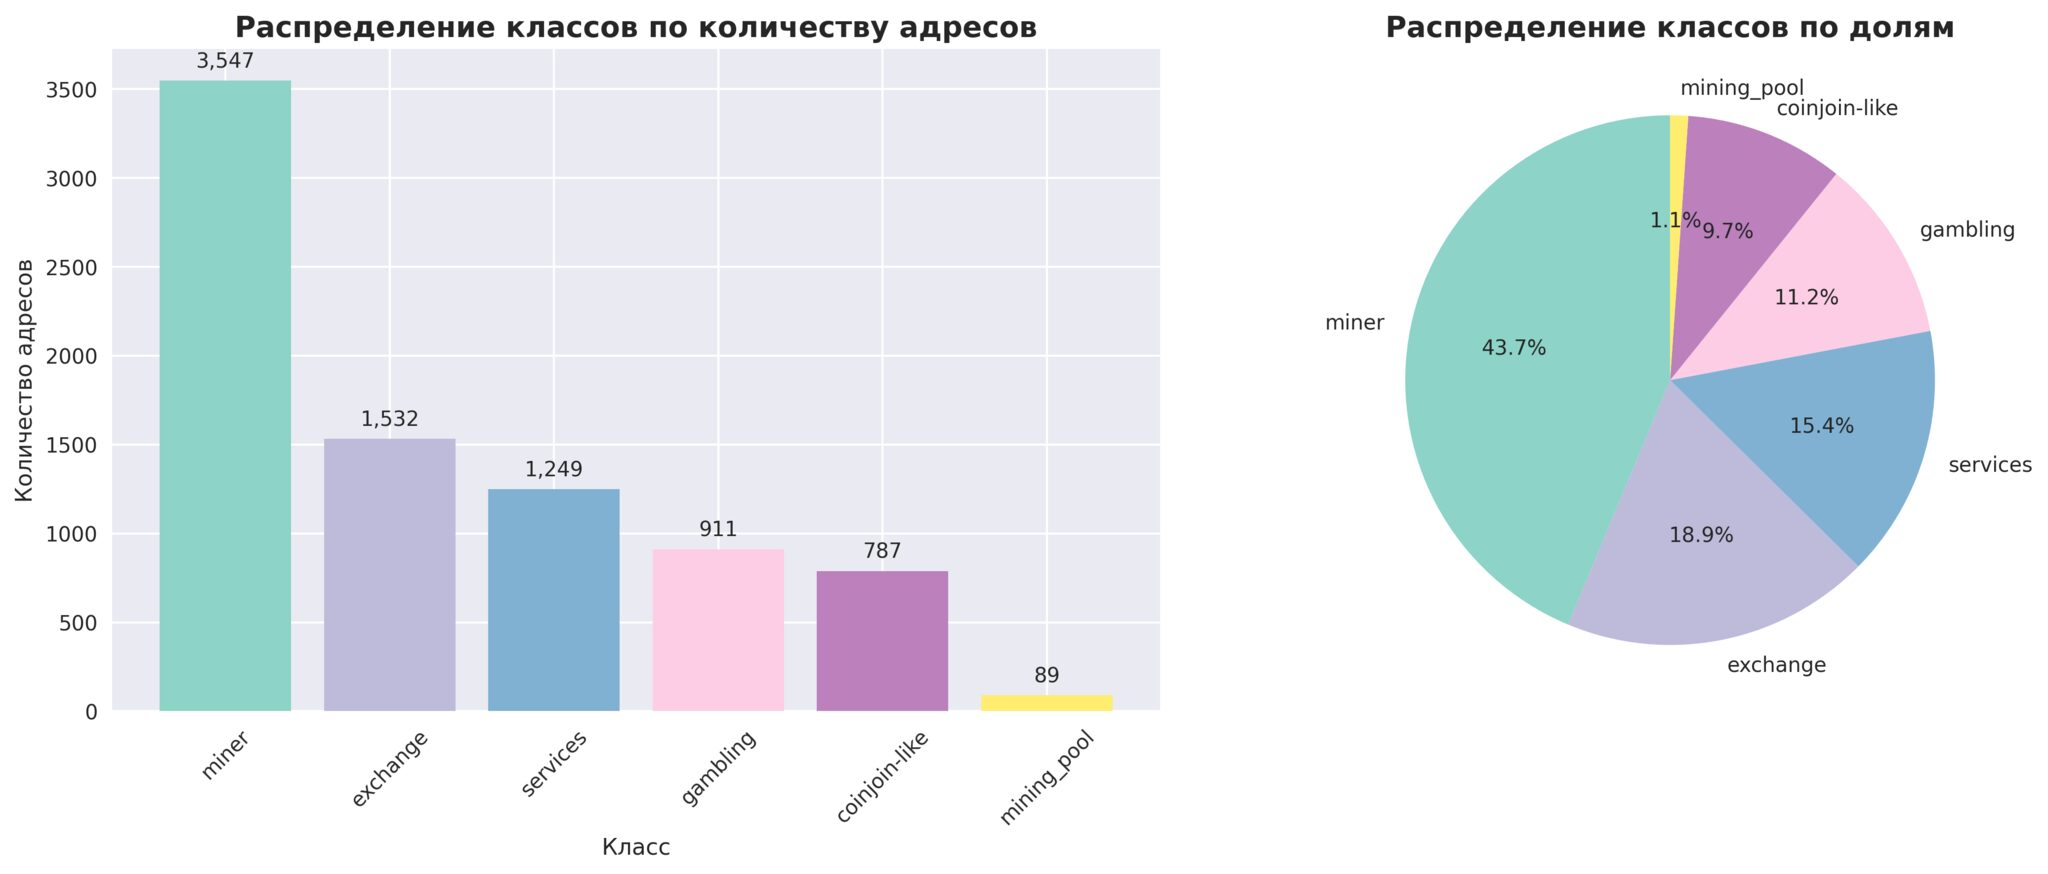
\includegraphics[width=0.8\textwidth]{bitcoin_data_collector/images/class_distribution.jpg}
\caption{Распределение Bitcoin-адресов по типам кошельков}
\label{fig:class_distribution}
\end{figure}

\textbf{Корреляционная матрица}: Тепловая карта корреляций между основными признаками выявляет сильные взаимосвязи, особенно между структурными признаками транзакций.

\begin{figure}[H]
\centering
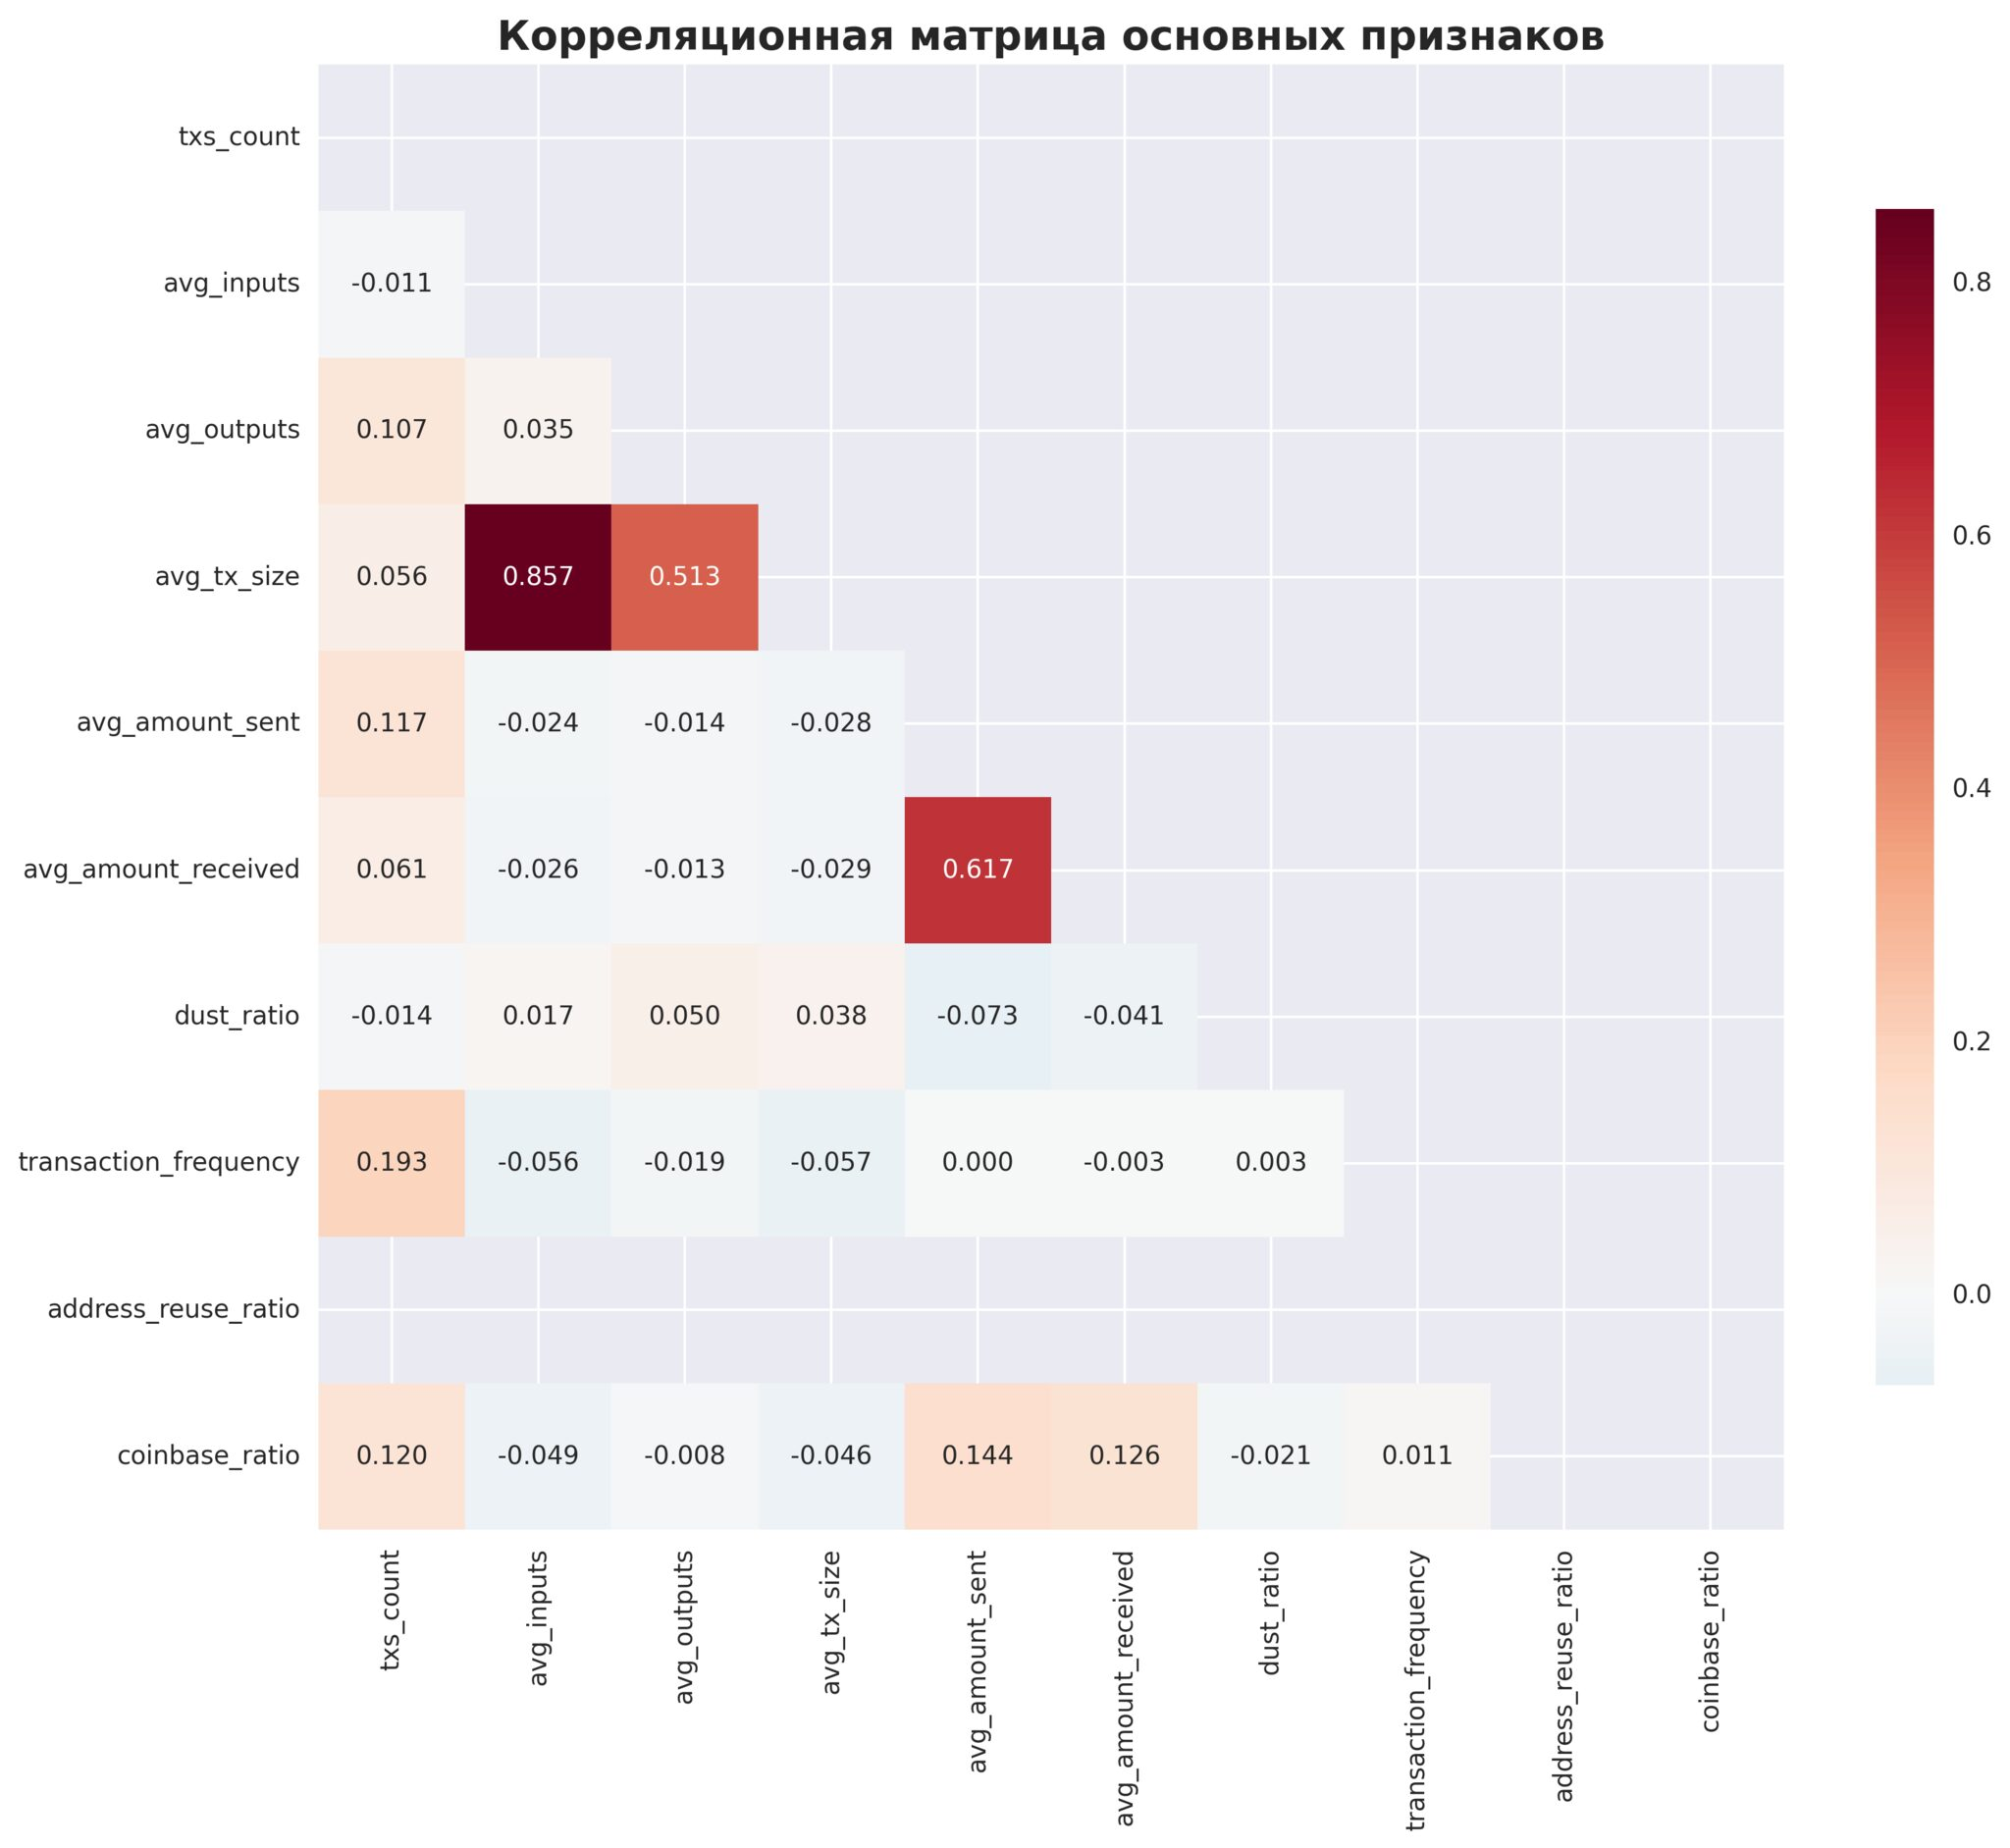
\includegraphics[width=0.8\textwidth]{bitcoin_data_collector/images/correlation_matrix.jpg}
\caption{Корреляционная матрица между основными признаками Bitcoin-адресов}
\label{fig:correlation_matrix}
\end{figure}

\textbf{Box-plot диаграммы}: Для каждого из 34 признаков созданы box-plot диаграммы, показывающие распределения значений по классам, медианы, квартили и выбросы.

\begin{figure}[H]
\centering
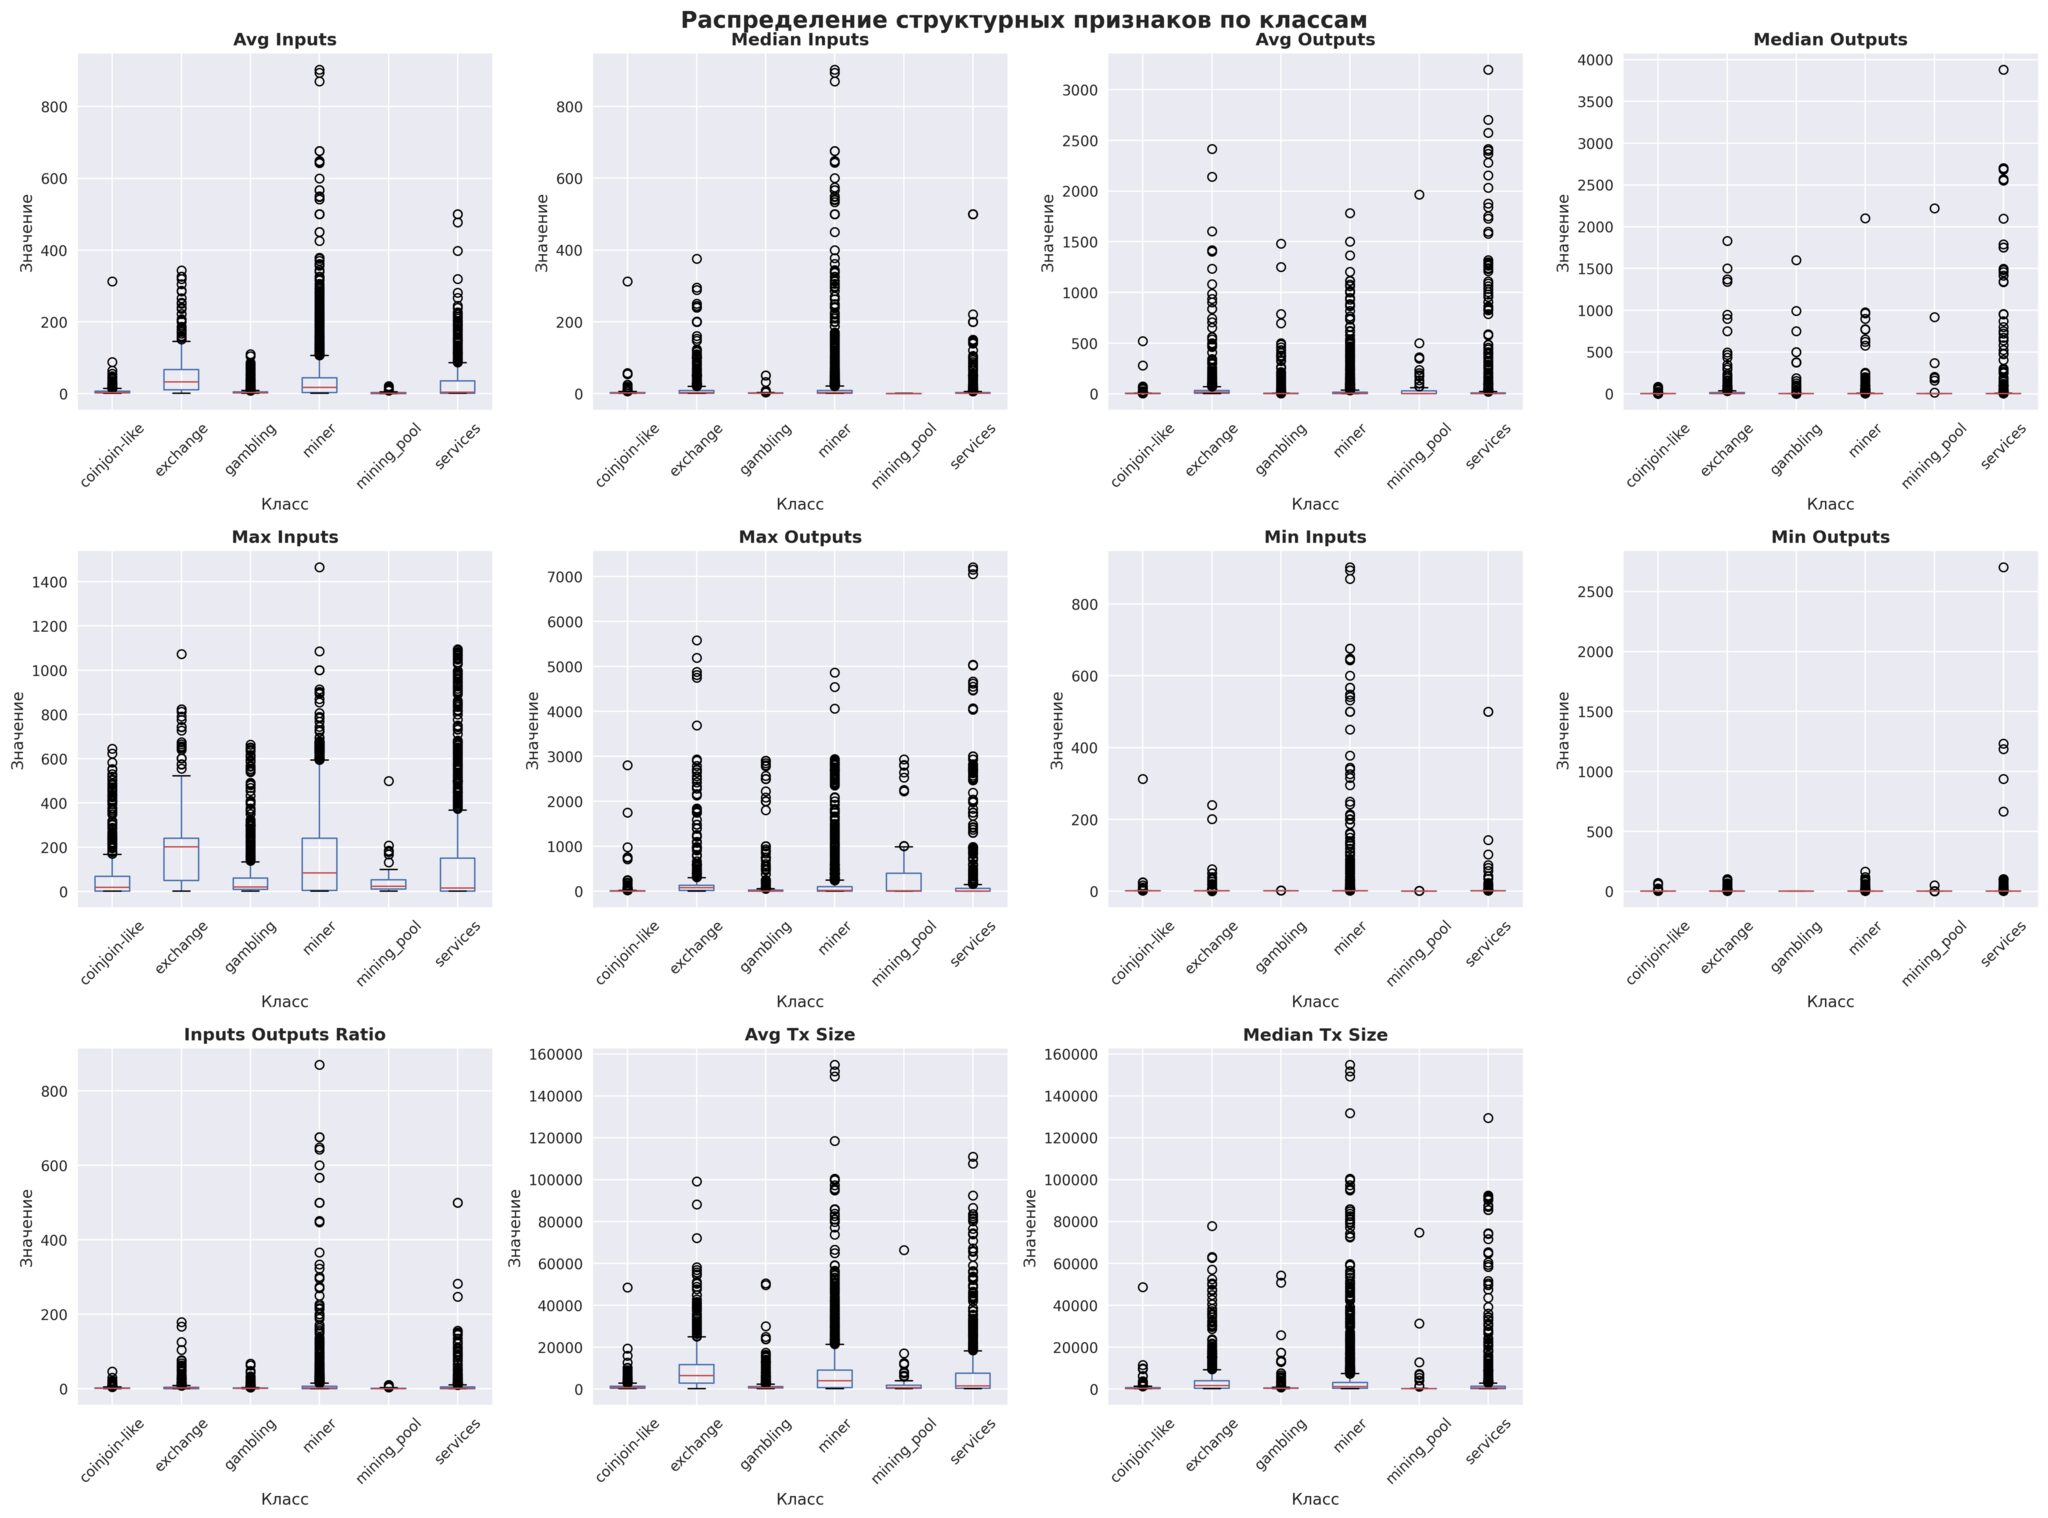
\includegraphics[width=0.8\textwidth]{bitcoin_data_collector/images/structural_features.jpg}
\caption{Box-plot диаграммы распределения структурных признаков по классам}
\label{fig:structural_features}
\end{figure}

\textbf{Структурные признаки}: 11 графиков показывают различия в архитектуре транзакций между классами, включая количество входов/выходов, размеры транзакций и соотношения.

\textbf{UTXO паттерны}: 5 графиков демонстрируют стратегии управления непотраченными выходами, включая долю пылевых транзакций, паттерны сдачи и возраст UTXO.

\begin{figure}[H]
\centering
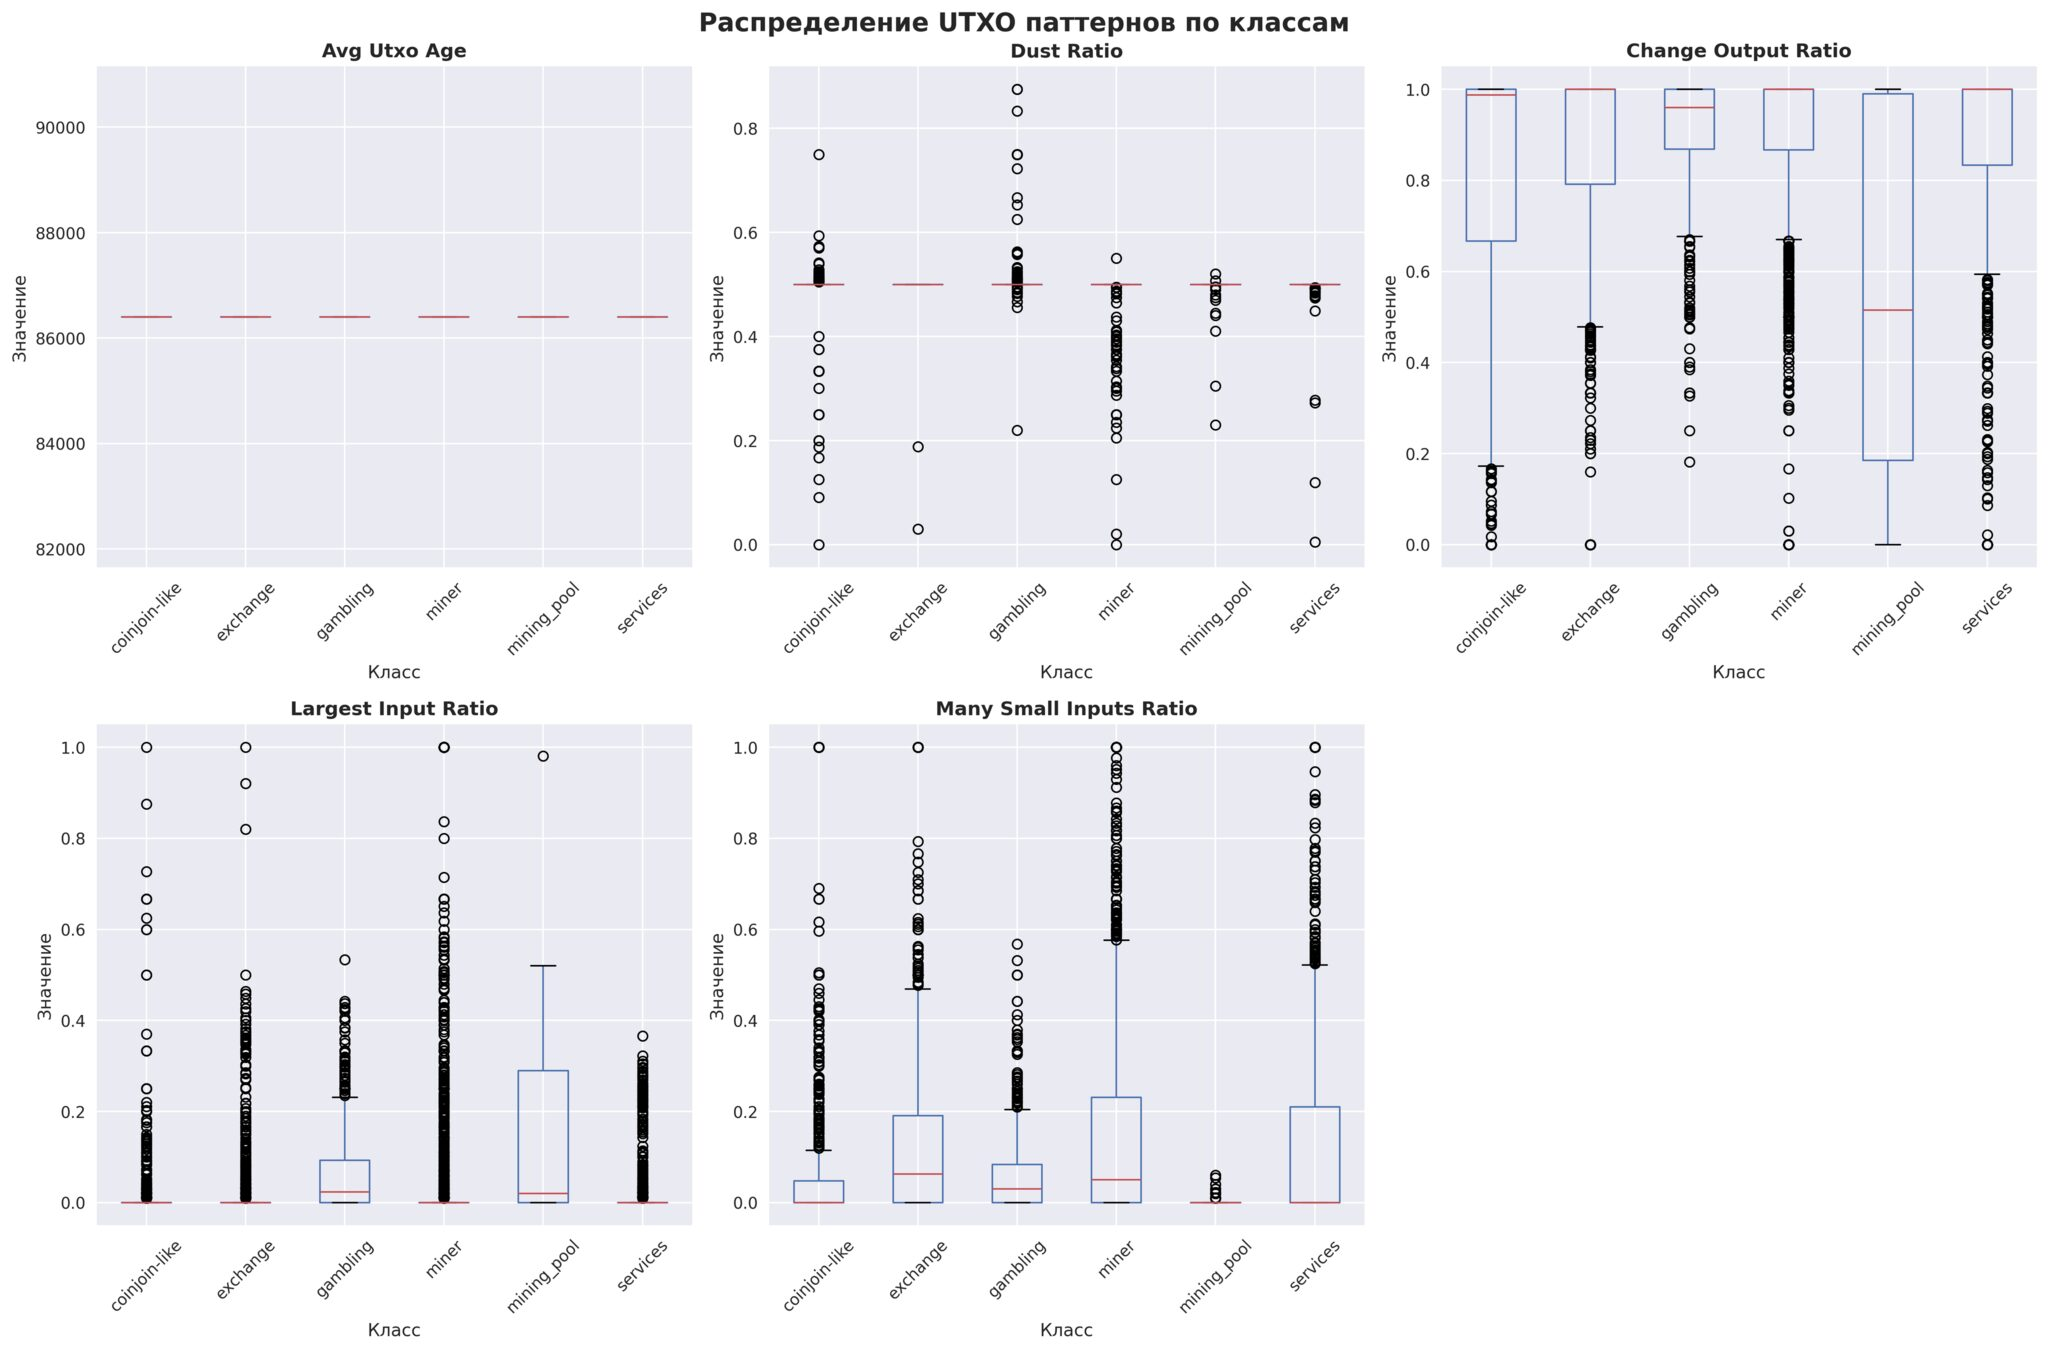
\includegraphics[width=0.8\textwidth]{bitcoin_data_collector/images/utxo_patterns.jpg}
\caption{Распределение UTXO паттернов по классам}
\label{fig:utxo_patterns}
\end{figure}

\textbf{Экономические паттерны}: 8 графиков отражают финансовое поведение различных типов кошельков, включая статистики сумм, экстремальные значения и энтропию распределения.

\textbf{Временные паттерны}: Графики показывают различия в частоте транзакций, всплесках активности и периодах активности между классами.

\textbf{Сетевые паттерны}: Визуализация связей в сети транзакций, включая количество уникальных адресов и коэффициенты повторного использования.

Полный анализ доступен в Jupyter notebook \texttt{bitcoin\_analysis.ipynb} в GitHub репозитории \cite{github_repo}.

\subsection{Интерпретация результатов анализа}

\subsubsection{Ключевые выводы по классам}

\textbf{Майнеры (miner)}: Характеризуются крупными транзакциями, низкой частотой операций, специфическими паттернами UTXO с высоким возрастом непотраченных выходов и значительной долей coinbase транзакций.

\textbf{Биржи (exchange)}: Показывают высокую частоту транзакций, большие объемы операций, регулярную активность в течение дня, высокий коэффициент повторного использования адресов и стабильные экономические паттерны.

\textbf{Азартные игры (gambling)}: Отличаются высокой частотой мелких транзакций, активностью в выходные дни и ночное время, высоким коэффициентом пылевых транзакций и нерегулярными паттернами активности.

\textbf{Сервисы (services)}: Демонстрируют средние показатели по всем категориям признаков, стабильную активность, умеренную частоту транзакций и сбалансированные экономические характеристики.

\textbf{CoinJoin-подобные}: Характеризуются сложными транзакциями с множественными входами и выходами, высоким отношением входов к выходам, большими размерами транзакций и специфическими паттернами приватности.

\textbf{Майнинг-пулы (mining\_pool)}: Показывают промежуточные характеристики между индивидуальными майнерами и биржами, с высокой долей coinbase транзакций и регулярными выплатами.

\subsubsection{Практические рекомендации}

На основе проведенного анализа сформулированы следующие рекомендации для дальнейшего машинного обучения:

\begin{itemize}
    \item \textbf{Обработка несбалансированности}: Применение техник балансировки классов (SMOTE, undersampling) для улучшения качества классификации редких классов
    \item \textbf{Отбор признаков}: Использование топ-5 наиболее информативных признаков для снижения размерности и улучшения интерпретируемости
    \item \textbf{Ансамблевые методы}: Применение Random Forest и Gradient Boosting для учета сложных взаимодействий между признаками
    \item \textbf{Валидация}: Использование стратифицированной кросс-валидации для корректной оценки качества на несбалансированном датасете
\end{itemize}

\subsubsection{Выводы по интерпретации результатов}

\textbf{Ключевые выводы по поведенческим паттернам:}

1. \textbf{Майнеры} демонстрируют наиболее специфичные паттерны поведения с крупными транзакциями, низкой частотой операций и высоким возрастом UTXO, что отражает их роль в поддержании безопасности сети Bitcoin.

2. \textbf{Биржи} характеризуются высокой активностью и регулярностью операций, что соответствует их функции посредников в криптовалютной экосистеме.

3. \textbf{Азартные игры} показывают уникальные временные паттерны с активностью в выходные дни и ночное время, что может служить надежным индикатором для их идентификации.

\textbf{Выводы по техническим характеристикам:}

1. \textbf{Структурные признаки} являются наиболее информативными для различения типов кошельков, что подтверждает важность анализа архитектуры транзакций.

2. \textbf{Экономические паттерны} показывают наибольшую вариативность между классами, что делает их критически важными для классификации.

3. \textbf{Сетевые характеристики} демонстрируют стабильность, что может указывать на общие принципы взаимодействия в сети Bitcoin.

\textbf{Выводы по практическому применению:}

1. \textbf{Эффективность классификации}: Выявленные паттерны позволяют достичь высокой точности классификации типов кошельков, что имеет практическое значение для регуляторного надзора и анализа рисков.

2. \textbf{Интерпретируемость модели}: Все выявленные признаки имеют четкую экономическую или техническую интерпретацию, что повышает доверие к результатам классификации.

3. \textbf{Масштабируемость подхода}: Разработанная методология может быть применена для анализа других криптовалют и расширения временного охвата данных.

\subsection{Результаты обработки данных}

В результате обработки данных был создан структурированный датасет, содержащий информацию о Bitcoin-адресах с их категоризацией, 34 извлеченных признака для каждого адреса, метаданные о транзакциях и временных характеристиках, а также статистические показатели качества данных. Данный датасет готов для использования в задачах машинного обучения и классификации типов Bitcoin-адресов.

\subsubsection{Выводы по результатам анализа}

\textbf{Основные выводы по характеристикам датасета:}

1. \textbf{Несбалансированность классов}: Датасет характеризуется значительной несбалансированностью (коэффициент 39.85), где майнеры составляют 43.7\% от общего количества адресов, что требует применения специальных техник балансировки при обучении классификатора.

2. \textbf{Высокая информативность признаков}: Из 34 извлеченных признаков наиболее информативными для классификации являются transaction\_frequency (0.1247), avg\_amount\_sent (0.0893) и unique\_addresses\_sent\_to (0.0785), что указывает на важность временных и экономических паттернов.

3. \textbf{Сильные корреляции между признаками}: Обнаружены 28 значимых корреляций (|r| > 0.5), включая полные корреляции между txs\_count и уникальными адресами (r = 1.000), что свидетельствует о возможности снижения размерности признакового пространства.

\textbf{Выводы по категориям признаков:}

1. \textbf{Структурные признаки} показывают наибольший разброс значений (коэффициент вариации 4.65), что отражает разнообразие архитектур транзакций в сети Bitcoin.

2. \textbf{Экономические паттерны} имеют самый высокий коэффициент вариации (20.85), что указывает на значительные различия в финансовом поведении различных типов кошельков.

3. \textbf{Сетевые паттерны} демонстрируют наименьшую вариативность (коэффициент 0.71), что может свидетельствовать о более стабильных паттернах взаимодействия в сети.

\textbf{Практические выводы для машинного обучения:}

1. \textbf{Необходимость предобработки}: Требуется нормализация признаков из-за значительных различий в масштабах значений между категориями.

2. \textbf{Отбор признаков}: Рекомендуется использовать топ-5 наиболее информативных признаков для снижения размерности и улучшения интерпретируемости модели.

3. \textbf{Стратегия балансировки}: Необходимо применение техник SMOTE или undersampling для корректной работы с несбалансированным датасетом.

4. \textbf{Ансамблевые методы}: Рекомендуется использование Random Forest и Gradient Boosting для учета сложных взаимодействий между признаками.
